\documentclass[a4paper]{article}
\usepackage{svn-multi}
% Version control information:
\svnidlong
{$HeadURL: https://practicas-derive.googlecode.com/svn/trunk/vectores.tex $}
{$LastChangedDate: 2008-11-13 12:37:02 +0100 (jue, 13 nov 2008) $}
{$LastChangedRevision: 3 $}
{$LastChangedBy: asalber $}
\svnid{$Id: vectores.tex 3 2008-11-13 11:37:02Z asalber $}
\pdfinfo{/CreationDate (D:\svnpdfdate)}
\svnRegisterAuthor{alf}{Alfredo Sánchez Alberca}

\usepackage[spanish]{babel}
\usepackage[utf8x]{inputenc}
\usepackage{amsmath}
\usepackage{macros}
\usepackage[dvips]{graphicx}
\usepackage{enumitem}
\usepackage{subfigure}
\usepackage[small,bf]{caption2}
\usepackage[top=3cm, bottom=3cm, left=2.54cm, right=2.54cm]{geometry}
\usepackage{fancyhdr}
\pagestyle{fancy}

\lhead{\textsc{Universidad San Pablo CEU}} \rhead{\textsl{\textsf{Departamento de Métodos Cuantitativos}}}
\renewcommand{\headrulewidth}{0pt}
\renewcommand{\floatpagefraction}{.8}
\renewcommand{\textfraction}{.1}
\setcaptionwidth{\textwidth} \addtolength{\captionwidth}{-40pt}
\captionstyle{indent} \setlength\captionindent{\parindent}

\makeatletter
\let\savees@listquot\es@listquot
\def\es@listquot{\protect\savees@listquot}
\makeatletter

\begin{document}
\sloppy
\practica{Práctica de Álgebra con DERIVE}{Vectores}

\bigskip
%\section*{Objetivos}
%El objetivo de esta práctica es aprender a manipular vectores y realizar las
%operaciones básicas del cálculo vectorial con Derive.

\section*{Fundamentos teóricos}
Los vectores son las estructuras elementales del Álgebra. Sus aplicaciones son múltiples sobre todo en el campo de la Física. En esta práctica se introduce el concepto de vector, tanto desde el punto de vista algebraico como geométrico, y se muestran las operaciones básicas del cálculo vectorial.

\subsection*{Escalares y vectores}
En álgebra y geometría se llama \emph{escalar} a cualquier magnitud que no tiene una dirección asociada, como por ejemplo el precio de un producto o la estatura de una persona. Y se llama \emph{vector} a cualquier magnitud que tiene asociada una dirección, como por ejemplo la velocidad de un móvil, que consta de dos elementos: su intensidad y su dirección. Utilizaremos la notación $\vec{u}$, $\vec{v}$, etc., para representar vectores. 

La magnitud de un vector $\vec{v}$ es lo que mide se conoce como \emph{módulo}
y se nota por $|\vec{v}|$, mientras que su dirección es el ángulo que forma
con respecto a un eje fijo que suele ser el eje horizontal.

\subsection*{Representación de vectores mediante coordenadas}
\subsubsection*{Coordenadas Cartesianas}
En geometría es común representar un vector como un segmento rectilíneo orientado, que queda determinado por dos puntos del espacio que son el origen y el final del vector. Un segmento orientado puede ubicarse en diferentes lugares dentro de un espacio $n$-dimensional. Sin embargo, con independencia de donde esté situado, si la longitud y la dirección no varían, dicho segmento representará siempre el mismo vector. Esto nos permitirá representar todos los vectores con un mismo origen, el origen en sistema de coordenadas cartesianas, tal y como se muestra en la figura~\ref{g:coordenadas}.

\begin{figure}[h!]
\begin{center}
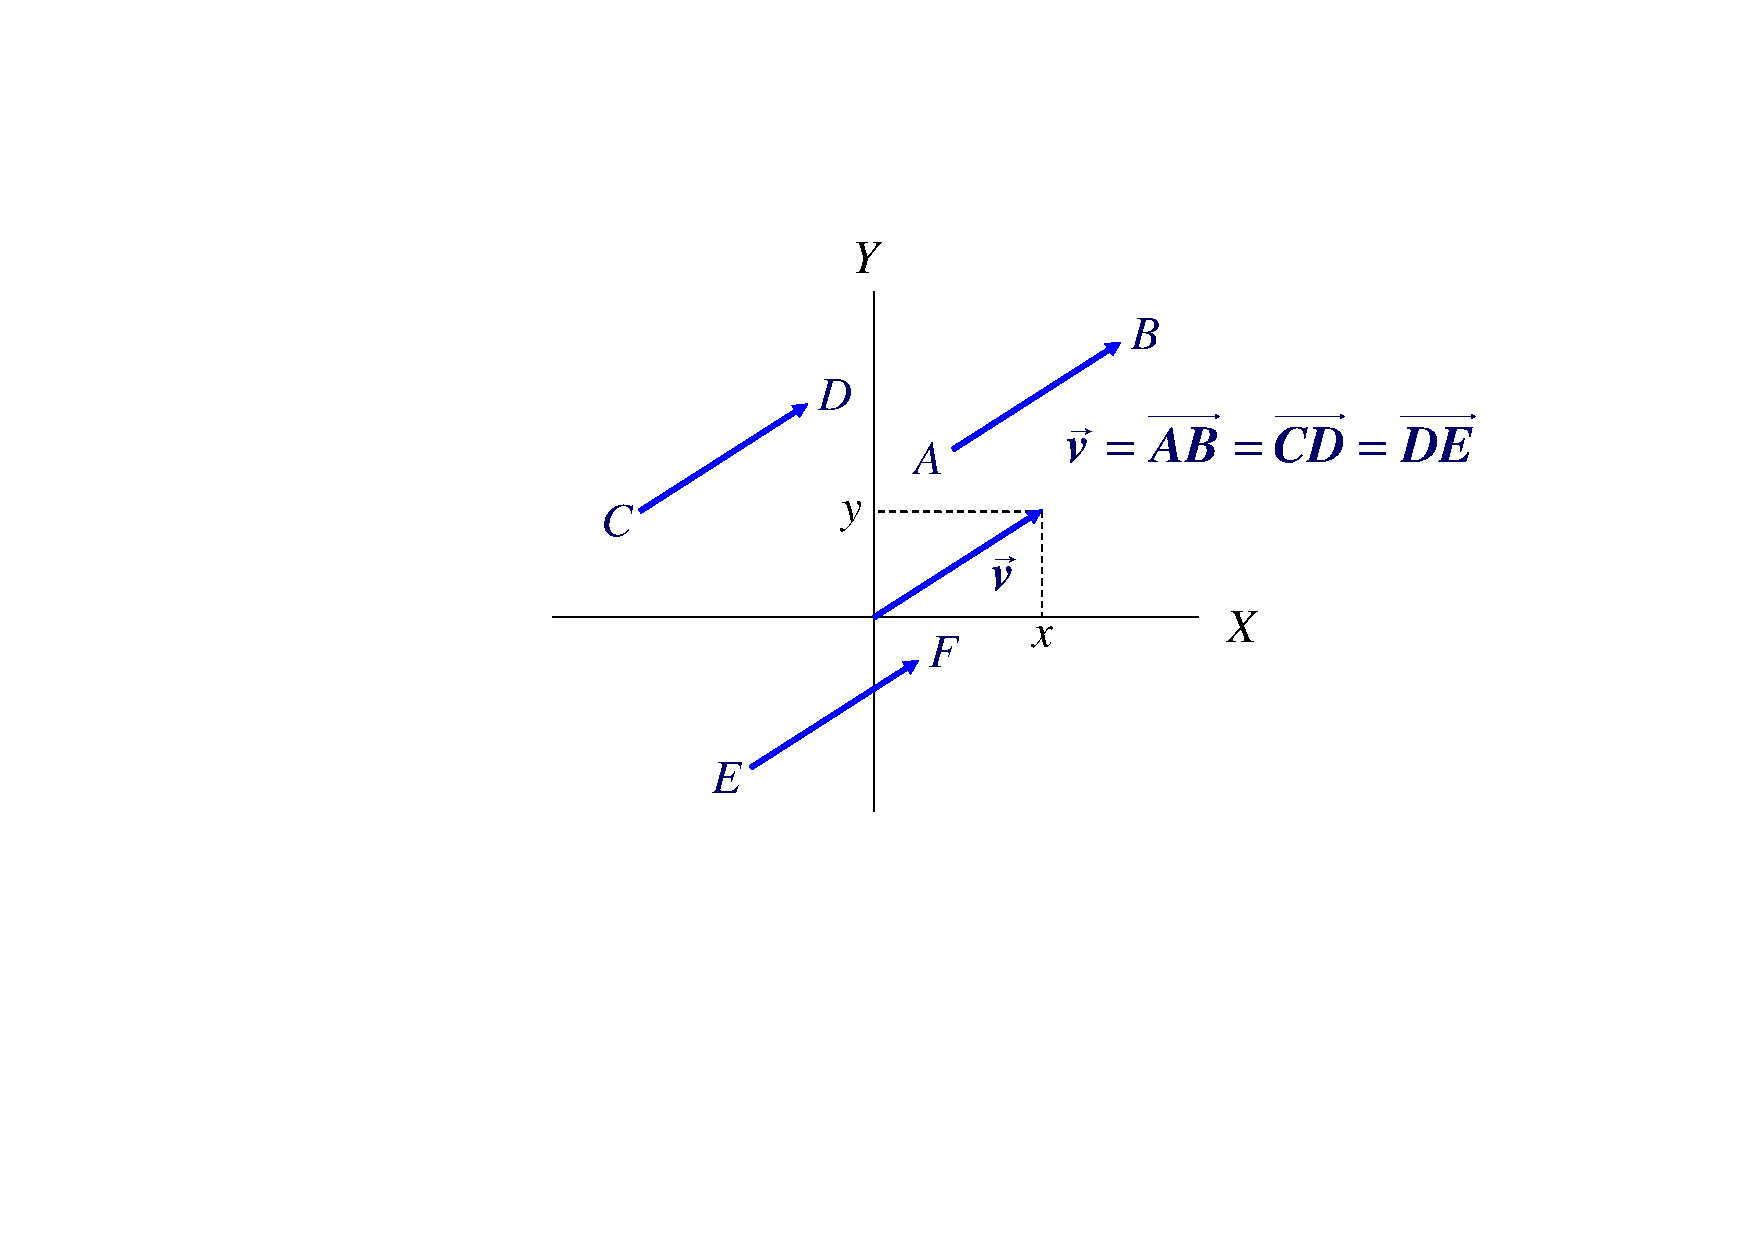
\includegraphics[scale=0.5]{coordenadas}
\caption{Representación de vectores mediante coordenadas en el plano real $\mathbb{R}^2$.}
\label{g:coordenadas}
\end{center}
\end{figure}

De este modo, un vector quedará unívocamente determinado por las coordenadas cartesianas del punto final del segmento, y utilizaremos dichas coordenadas para representarlo, según se ilustra en la figura~\ref{g:coordenadascartesianas}. 

\subsubsection*{Coordenadas polares}
Otra forma habitual de representar un vector en el plano real $\mathbb{R}^2$ es mediante su módulo, que nos indica su magnitud, y el ángulo que forma con el eje de abscisas, que nos indica su dirección, tal y como se ve en la figura~\ref{g:coordenadaspolares}.

\begin{figure}[h!]
\centering \subfigure[Coordenadas cartesianas.] {\label{g:coordenadascartesianas}
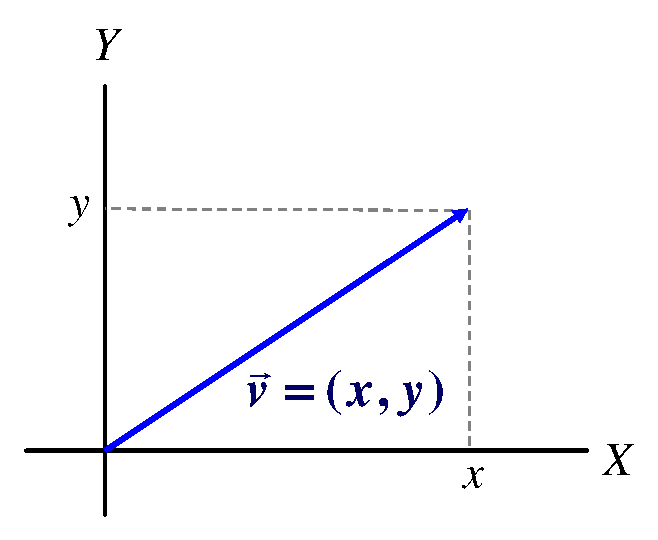
\includegraphics[scale=0.5]{coordenadascartesianas}}\qquad
\subfigure[Coordenadas polares.]{\label{g:coordenadaspolares}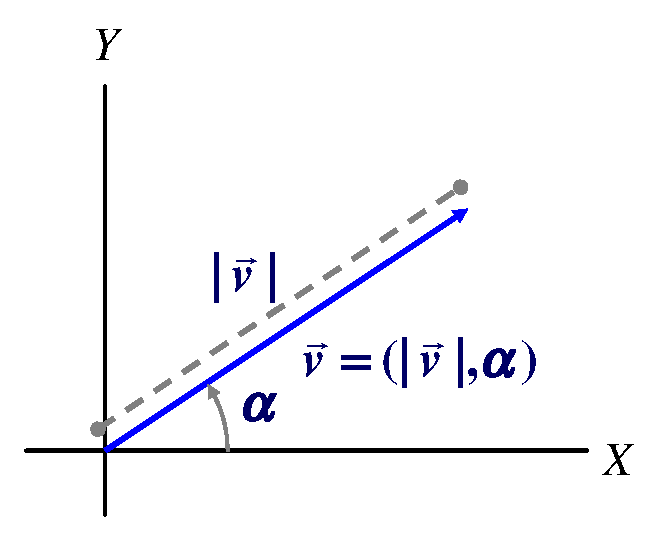
\includegraphics[scale=0.5]{coordenadaspolares}}
\caption{Representación de vectores en el plano real $\mathbb{R}^2$ mediante distintos tipos de coordenadas.}
\end{figure}  

\subsection*{Tipos de vectores}
\begin{description}
\item [Vector nulo] Es el vector $\vec{0}=(0,\ldots,0)$ cuyas coordenadas valen
todas 0.
\item [Vector unitario] Es un vector con módulo 1.
\item [Vector opuesto] Es el vector que tiene las mismas coordenadas que el original pero con signo contrario.
\item [Vectores paralelos] Son dos vectores que tienen la misma dirección y por
tanto forman un ángulo nulo.
\item [Vectores ortogonales] Son dos vectores que tienen direcciones
perpendiculares y por tanto forman un ángulo de 90 grados.
\item [Vectores ortonormales] Son dos vectores ortogonales que además son
unitarios.
\end{description}

\subsection*{Operaciones con vectores}
Dados dos vectores $\vec{u},\vec{v}\in \mathbb{R}^n$ con
$\vec{u}=(u_1,\ldots,u_n)$ y $\vec{v}=(v_1,\ldots,v_n)$, y un escalar $a\in
\mathbb{R}$, se definen las siguientes operaciones vectoriales:
\begin{description}
\item [Suma de vectores]
\[
\vec{u}+\vec{v}=(u_1,\ldots,u_n)+(v_1,\ldots,v_n)=(u_1+v_1,\ldots,u_n+v_n).
\]

Al sumar dos vectores obtenemos otro vector cuyas coordenadas son la suma de las coordenadas de los vectores sumandos (figura~\ref{g:suma}).

\item [Producto de un vector por un escalar]
\[
a\vec{v}=a(v_1,\ldots,v_n)=(av_1,\ldots,av_n).
\]

Al multiplicar un vector por un escalar, obtenemos otro vector con la misma
dirección que el vector original, pero con su módulo multiplicado por dicho
escalar (\ref{g:producto}). De esta manera, resulta sencillo obtener vectores unitarios en la
misma dirección que uno dado $\vec{v}$, sin más que dividirlo por su módulo
\[\frac{\vec{v}}{|\vec{v}|}.\]

\begin{figure}[h!]
\centering \subfigure[Suma de vectores.] {\label{g:suma}
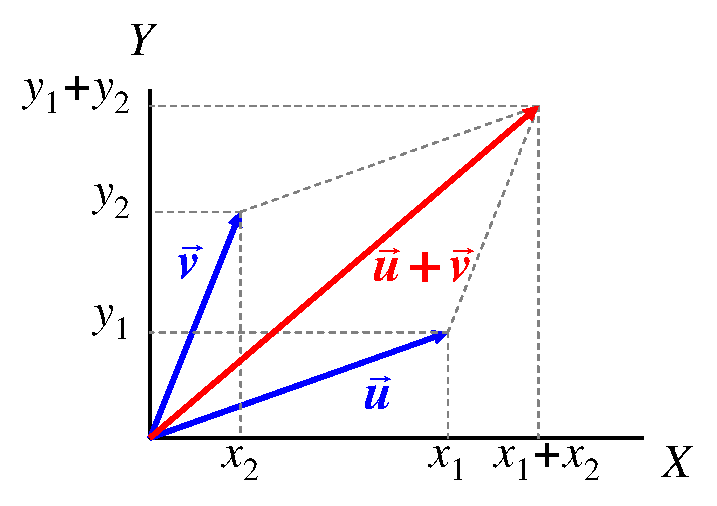
\includegraphics[scale=0.6]{suma}}\qquad
\subfigure[Producto de un vector por un escalar.]{\label{g:producto}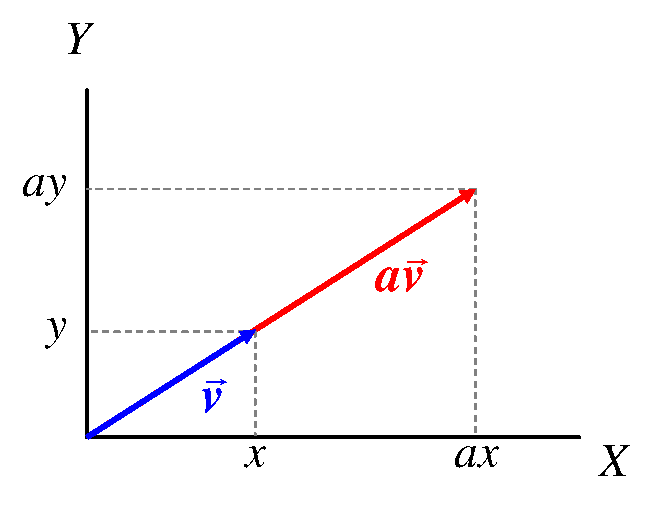
\includegraphics[scale=0.6]{producto}}
\caption{Operaciones con vectores en el plano real $\mathbb{R}^2$.}
\end{figure}  

\item [Producto escalar de vectores]
\[
\vec{u}\cdot\vec{v}=(u_1,\ldots,u_n)\cdot(v_1,\ldots,v_n)=u_1v_1+\cdots+u_nv_n.
\]
Geométricamente, resulta sencillo comprobar que
\[
\vec{u}\cdot\vec{v}=|\vec{u}||\vec{v}|\cos\alpha, \] donde $\alpha$ es el
ángulo que forman $\vec{u}$ y $\vec{v}$, y en el caso de que $\vec{u}$ y
$\vec{v}$ sean vectores unitarios, se tiene $\vec{u}\cdot\vec{v}=\cos\alpha$.
De este modo, el producto escalar de dos vectores resulta muy útil para obtener
información sobre el ángulo $\alpha$ que forman, y tiene importantes
aplicaciones.

Una aplicación inmediata es el cálculo del módulo de un vector, ya que se
cumple
\[ \vec{v}\cdot\vec{v}=|\vec{v}||\vec{v}|\cos 0=|\vec{v}|^2.\]

Por otro lado, el producto escalar nos da una condición muy importante para
verificar si dos vectores no nulos $\vec{u}$ y $\vec{v}$ son ortogonales, ya
que en tal caso
\[
\vec{u}\cdot\vec{v}=|\vec{u}||\vec{v}|\cos \frac{\pi}{2}=0.\]

Otra aplicación muy útil es el cálculo de la proyección de un
vector $\vec{u}$ sobre otro $\vec{v}$. Tal y como se muestra en la figura~\ref{g:proyeccion}, el
módulo será
\[|\vec{u}|\cos\alpha=\frac{\vec{u}\cdot\vec{v}}{|\vec{v}|},
\]
y la dirección será la misma que la del vector $\vec{v}$. Así pues, podemos
obtener fácilmente el vector proyección multiplicando su módulo por el vector
unitario en la dirección de $\vec{v}$, es decir
\[
\frac{\vec{u}\cdot\vec{v}}{|\vec{v}|}\frac{\vec{v}}{|\vec{v}|}=
\frac{\vec{u}\cdot\vec{v}}{\vec{v}\cdot\vec{v}}\vec{v}.
\]

\begin{figure}[h!]
\begin{center}
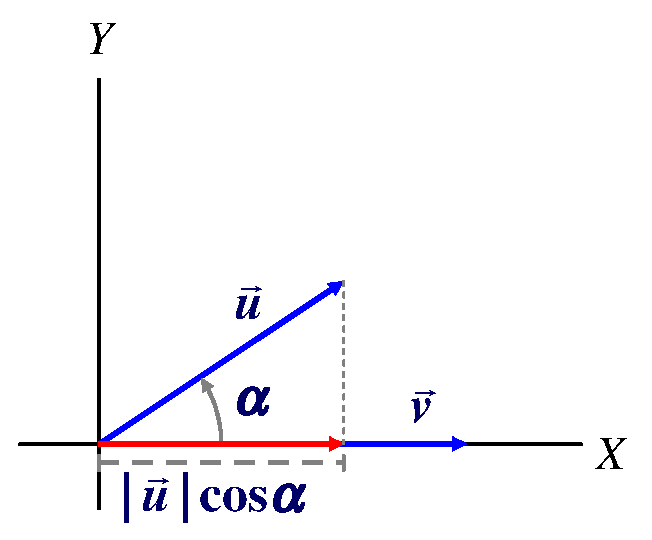
\includegraphics[scale=0.5]{proyeccion}
\caption{Proyección de un vector sobre otro en el plano real $\mathbb{R}^2$.}
\label{g:proyeccion}
\end{center}
\end{figure}

\item [Producto vectorial de vectores] Si además, $\vec{u}$ y $\vec{v}$ son vectores
de un espacio tridimensional, como por ejemplo $\vec{u},\vec{v}\in \mathbb{R}^3$,
\[
\vec{u}\times\vec{v}=(u_1,u_2,u_3)\times(v_1,v_2,v_3)=(u_2v_3-u_3v_2,u_3v_1-u_1v_3,u_1v_2-u_2v_1).
\]
El producto vectorial origina un nuevo vector perpendicular al plano formado
por $\vec{u}$ y $\vec{v}$ y con módulo
$|\vec{u}\times\vec{v}|=|\vec{u}||\vec{v}|\sen \alpha$, donde $\alpha$ es el
ángulo que forman forman $\vec{u}$ y $\vec{v}$. Geométricamente, el módulo del
producto vectorial nos da el área del paralelogramo formado por $\vec{u}$ y
$\vec{v}$.

\end{description}

\section*{Ejercicios Prácticos}
\begin{enumerate}[leftmargin=*]
\item Sean $\vec{u}=(1,2,3)$, $\vec{v}=(-1,1,0)$ y $\vec{w}=(a,b,c)$, tres
vectores de $\mathbb{R}^3$. Se pide:
\begin{enumerate}
\item Definir dichos vectores en Derive (menú \texttt{Author->Vector}) y calcular su
módulo ( utilizar la función \texttt{Abs}).
\item Calcular los siguientes vectores:
\begin{enumerate}
\item $\vec{u}+\vec{v}$.
\item $\vec{u}+\vec{w}$. ¿Cuánto deben valer $a$, $b$ y $c$ para que $\vec{u}$
y $\vec{w}$ sean opuestos?
\item $\vec{u}+2\vec{v}-3\vec{w}$.
\end{enumerate}
\item Calcular vectores unitarios correspondientes a $\vec{u}$ y $\vec{v}$.
\item Calcular los siguientes productos escalares:
\begin{enumerate}
\item $\vec{u}\cdot\vec{v}$.
\item $\vec{v}\cdot\vec{w}$. ¿Qué valores de $a$, $b$ y $c$ nos darían un
vector ortogonal a $\vec{v}$? ¿Son los vectores obtenidos ortonormales?
\item $2\vec{w}\cdot\vec{v}$.
\item $(2\vec{w}+\vec{u})\cdot 5\vec{v}$.
\end{enumerate}
\item Calcular de nuevo el módulo de $\vec{u}$, $\vec{v}$ y $\vec{w}$ haciendo
uso del producto escalar.

\item Calcular el ángulo en radianes que forman los siguientes vectores:
\begin{enumerate}
\item $\vec{u}$ y $\vec{v}$.
\item $(2\vec{u}+\vec{w})$ y $\vec{v}$.
\end{enumerate}

\item Calcular el vector proyección de los siguientes vectores:
\begin{enumerate}
\item $\vec{u}$ sobre $\vec{v}$.
\item $\vec{v}$ sobre $\vec{u}$.
\item $\vec{w}$ sobre $\vec{v}$.
\end{enumerate}

\item Calcular los siguientes productos vectoriales (utilizar la función \texttt{Cross}):
\begin{enumerate}
\item $\vec{u}\times\vec{v}$.
\item $\vec{v}\times\vec{w}$.
\item $(2\vec{w}+\vec{u})\times \vec{u}$.
\end{enumerate}
\end{enumerate}
\item Dados los vectores $\vec{u}=(1,2)$ y $\vec{v}=(-3,4)$ en coordenadas cartesianas, dar su representación en coordenadas polares.
\item Dados los vectores $\vec{u}=(1,\pi/4)$ y $\vec{v}=(2,-2\pi/3)$ en coordenadas polares, dar su representación en coordenadas cartesianas.
\end{enumerate}

\section*{Problemas}
\begin{enumerate}[leftmargin=*]
\item Sean $\vec{u}=(3,2,1,0)$, $\vec{v}=(-1,2,0,-2)$ y $\vec{w}=(a,b,c,d)$, tres
vectores de $\mathbb{R}^3$. Se pide:
\begin{enumerate}
\item ¿Qué vector tiene mayor magnitud $\vec{u}$ o $\vec{v}$?
\item Calcular los siguientes vectores:
\begin{enumerate}
\item $\vec{u}+\vec{v}$.
\item $\vec{u}-\vec{w}$.
\item $\vec{u}-3\vec{v}+\vec{w}$.
\end{enumerate}
\item Calcular vectores unitarios correspondientes a $\vec{u}$ y $\vec{v}$.
\item Calcular los siguientes productos escalares:
\begin{enumerate}
\item $\vec{u}\cdot\vec{v}$. ¿Son estos vectores ortogonales? 
\item $\vec{v}\cdot\vec{w}$.
\item $2\vec{w}\cdot\vec{v}$.
\item $(2\vec{w}+\vec{u})\cdot 5\vec{v}$.
\end{enumerate}

\item Construir un vector ortonormal a $\vec{u}$ y otro a $\vec{v}$.

\item Calcular de nuevo el módulo de $\vec{u}$, $\vec{v}$ y $\vec{w}$ haciendo
uso del producto escalar.

\item Calcular el ángulo en radianes que forman los siguientes vectores:
\begin{enumerate}
\item $\vec{u}$ y $\vec{v}$.
\item $(\vec{u}-3\vec{w})$ y $\vec{v}$.
\end{enumerate}

\item Calcular el vector proyección de los siguientes vectores:
\begin{enumerate}
\item $\vec{u}$ sobre $\vec{v}$.
\item $\vec{v}$ sobre $\vec{u}$.
\item $\vec{w}$ sobre $\vec{v}$.
\end{enumerate}

\end{enumerate}

\end{enumerate}
\end{document}
